\subsection{Infrastructure Specifications}

\subsubsection{Infrastructure Overview}
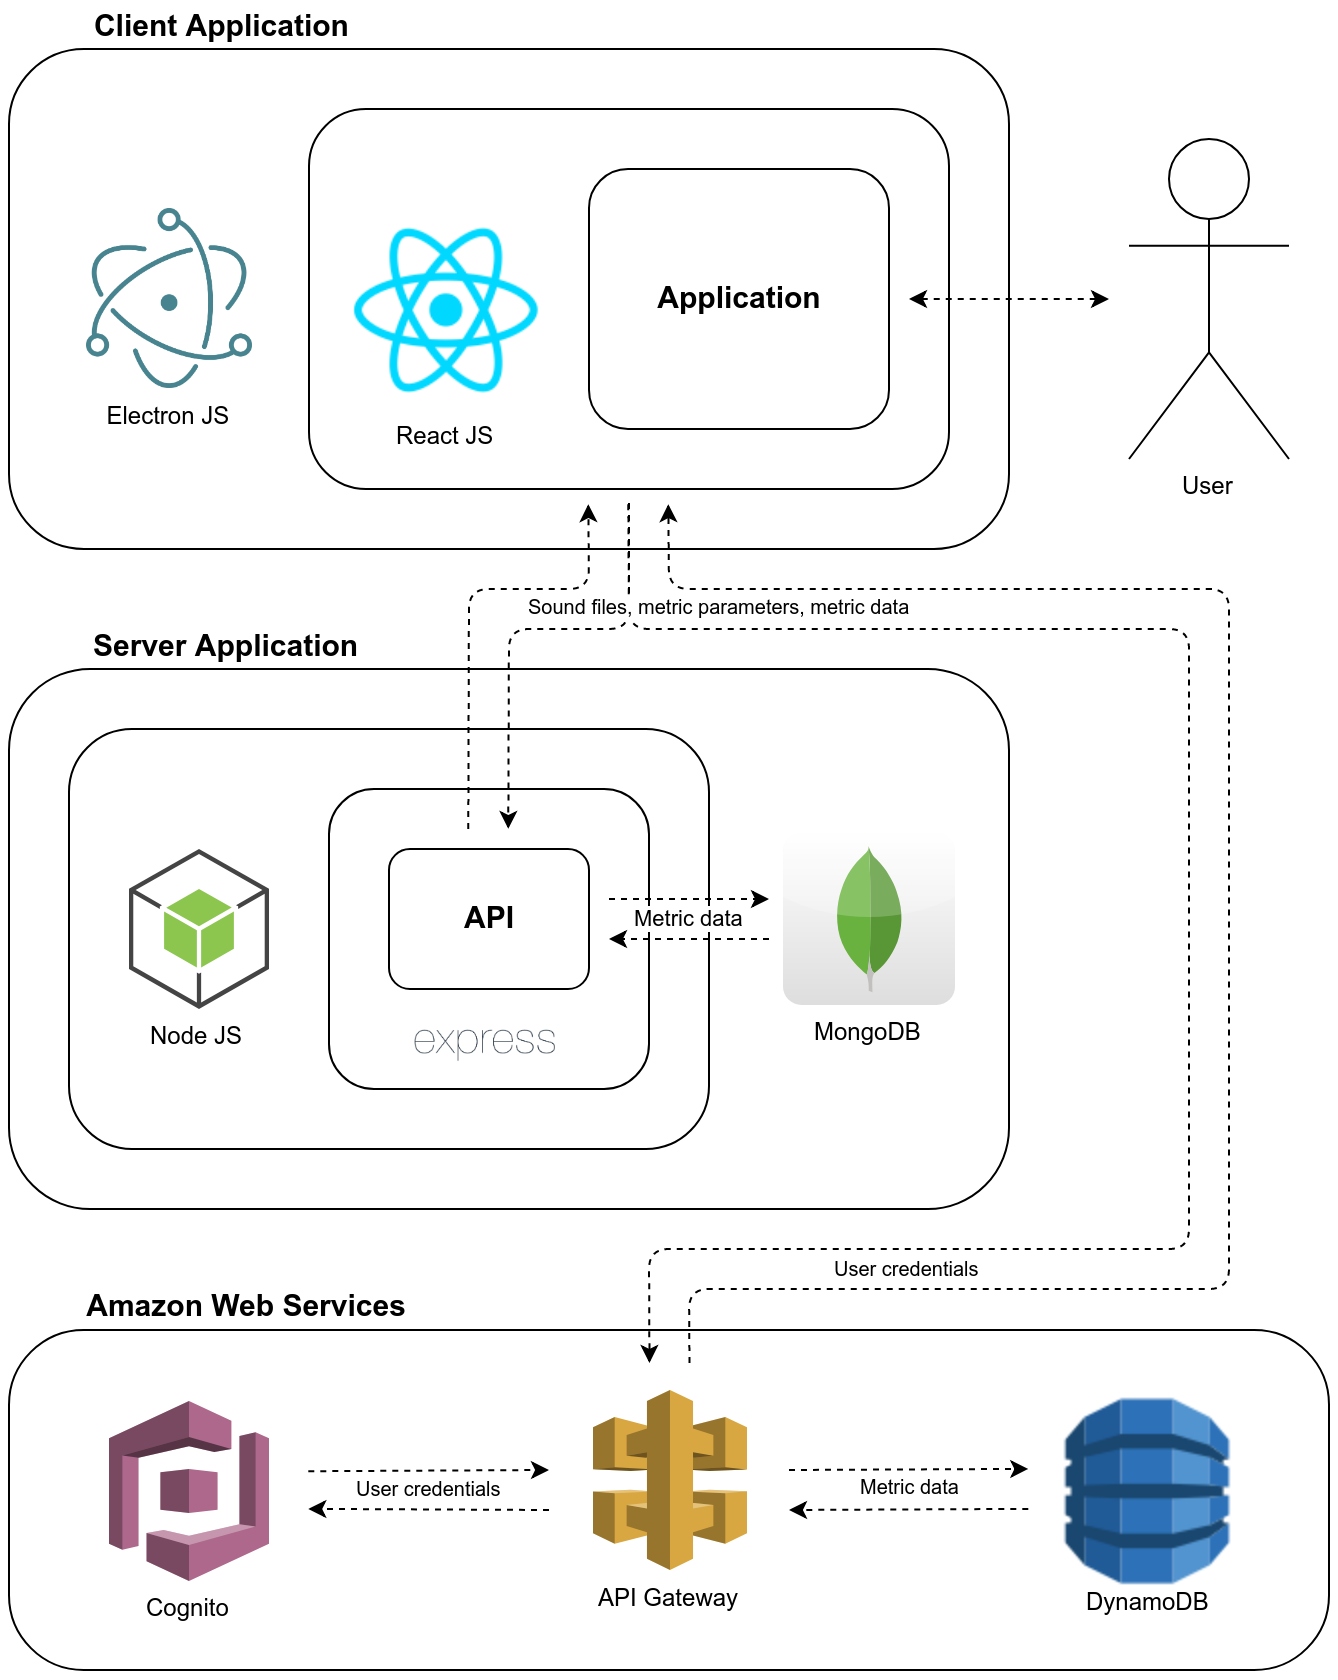
\includegraphics[width=\textwidth]{InfrastructureOverview}
At a high level, the system\textquotesingle s infrastructure is composed of three main parts:
\begin{enumerate}
    \item The \textbf{Client Application}: This contains the user interface with which any users may interact. It runs via an Electron application, and so will be able to run on all major operating systems. Using this application, a user may log into an account, create job requests to process audio files, and present the results of those jobs in a visually accessible manner.
    \item The \textbf{Server Application}: This is where the vast majority of the heavy lifting occurs, including the analysis of audio files for metric data, the storage of the resulting data, and the transmission of any files or data requested by the user via the Client Application. Typically, this application runs on a dedicated server, on which any sound files that are to be analyzed are stored. However, it is equally as possible for the user to run this application and the Client Application on the same machine.
    \item \textbf{Amazon Web Services}: AWS will be tasked with user account management, metric data storage, and intercommunication between Client and Server Applications over the internet. Users that run their own instances of the Server Application will be able to enable data sharing from their own servers, the data from which will be mirrored on AWS DynamoDB, accessible by other users from across the web.
\end{enumerate}

\subsubsection{Front End Infrastructure}
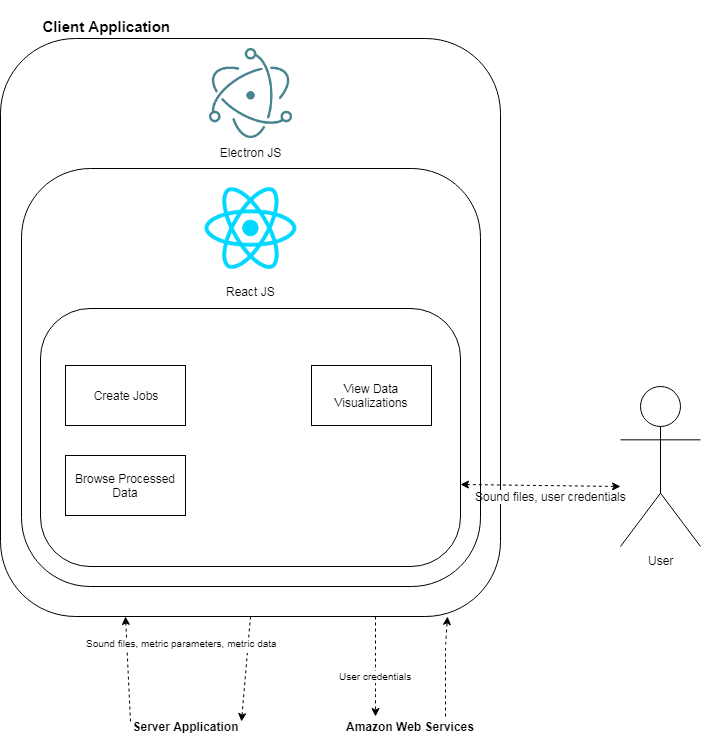
\includegraphics[width=\textwidth]{ClientInfrastructure} \\
The diagram above explains some of the functionality of the client frontend. The specific pages and their design can be seen in the User Interface Specifications section of this report. The frontend is where the user will be spending their time analyzing data and sharing results. The core functionalities of the frontend include creating jobs, browsing processed data, viewing data visualizations, creating public server access for collaboration, and creating research groups.\par
Creating jobs is the process of the user specifying a set of sound files, and the indices and parameters they wish to run on them. As explained in the backend specifications, the outputs are passed to the local database, and used to present the data in visualizations for the user. A user will create a job by selecting sound files whether locally or on their server space, and adding one or more index options and their respective parameters. If the user does not wish to specify parameters, a set of preset values will be used. If the user does not wish to specify an index, then all of the indices will be analyzed. Additionally, the user can create preset index and paremeter sets that they may use frequently, and simply use that set to analyze the data set.\par
As the user analyzes data over time, the results will be stored on the local database, and possibly the remote database should they choose to publish their results for collaboration. Using our service, the user can browse through their processed data to see what analysis they have done on what data sets. From here, they can also look at visualizations.\par
Our service will provide built in data visualization tools. Looking at change of index values over time is important to researchers to see how recent weather events or human interactions have affected the local wildlife. Another visualization available is a line graph, showing the index values by sound file over the whole data set. This is useful to researchers for identifying outliers, as they can easily see which sound files contained a much higher or lower index compared to the rest of the data set. As for collaboration, a geographic heat map is planned to help show where research is being done, as well as the kind of index values being observed at these locations.\par
The more simple side of the front end includes creating research groups and providing public server access. A user can create a research group, making them the admin. They then can add other users to their group, as well as promote members to admin. Research groups allow users access to other members\textquotesingle\ analyzed data and visualizations. As for public server access, our sponsor mentioned how it can be difficult to easily share sound files and data analysis with other researchers across the country. We are going to provide multiple ways for users to do this easily through our service. By implementing OneDrive, Google Drive, and DropBox into our service, users can provide public access folders for hosting sound files and analysis they wish to openly share. In addition, we also will allow users to upload private server credentials that our service will utilize to allow others access to the server for viewing whatever has been made public.

\subsubsection{Local Backend Infrastructure}
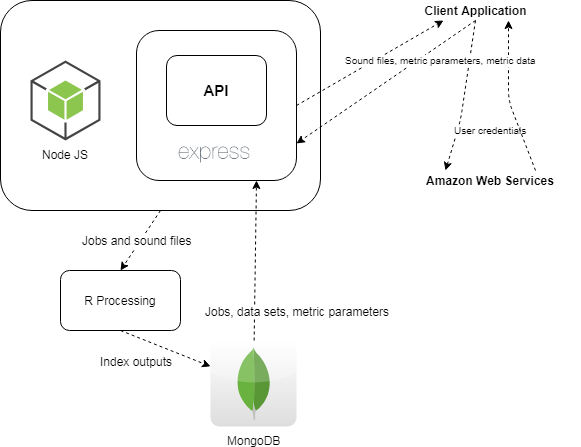
\includegraphics[width=\textwidth]{ServerInfrastructure} \\
This diagram goes into a bit more detail on the local backend. Using Express, our API is constructed to help the backend(s) and frontend communicate, all wrapped in a Node JS application. The front end orchestrates the user\textquotesingle s inputs and jobs to be run, which are then processed in the location the user has specified. This could be a local server that the user has set up using our server side application, or it could be their desktop computer. These jobs and input files go through the R scripts included for analysis in the soundecology package, depending on the user specified indices to be processed.\par
After the analysis is done, the output is different for each index. The MongoDB database we have constructed is set up specifically for storing each index\textquotesingle s output(s). See the database specifications for more a more in depth explanation of that infrastructure.\par
Once the data is stored in the local database, it is then accessible in the user interface on the frontend. We consider this implementation to be perfect for our system, as the local database can be kept on either the user\textquotesingle s desktop or on their server. If the database is hosted on the server, then any other researcher in the network can access this database and see analysis from a peer. This is important for the collaboration requirement made by our sponsor.

\subsubsection{Remote Backend Infrastructure}
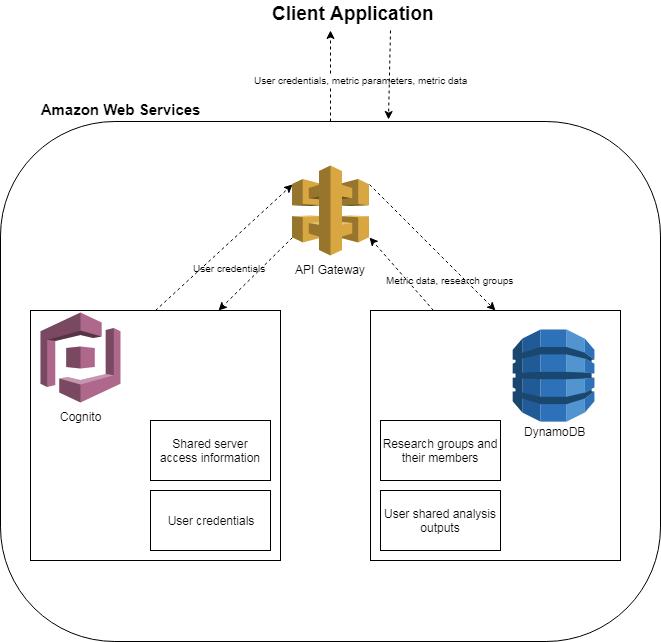
\includegraphics[width=\textwidth]{AWSOverview} \\
Using Amazon Web Services, we can use DynamoDB and Cognito to securely and efficiently manage our users\textquotesingle\ credentials and analysis. Cognito is used for storing user credentials and DynamoDB for research groups and their respective permissions, as well as user shared data.\par
Amazon Cognito is a very useful tool, as it provides a built in interface for users to create accounts as well as log in to existing accounts. These credentials are then stored securely by Amazon to easily create user pools. In addition, Cognito allows for Facebook and Google account log ins, to make account creation easier for the user.\par
DynamoDB is a non relational database, which is useful for us because our local MongoDB database is also non relational. The DynamoDB service will store user shared data analysis that they did on their desktop application. From here, anyone using the service can see that researcher\textquotesingle s analysis. In addition to data outputs, this service will store the user created research groups and their members in order to ensure that users are able to collaborate \textbf{only} with those they wish to.
